\subsubsection{Ciclo de vida}
    El ciclo de vida de los mixomicetos es muy complejo, y se divide en dos fases: 
        la fase vegetativa y la fase reproductiva.
    \vskip 0.5cm
    % Parrafo 5
    La fase vegetativa se divide en 3 etapas:
    \begin{itemize}
        \item \textbf{Etapa de alimentaci\'on}: En esta etapa, las c\'elulas individuales 
            se mueven por medio de seud\'opodos o flagelos, y se alimentan de bacterias, 
            levaduras y otros microorganismos que se encuentran en el suelo.
        \item \textbf{Etapa de crecimiento}: En esta etapa, las c\'elulas individuales 
            se fusionan para formar un plasmodio, que es una masa de citoplasma multinucleado 
            sin separaci\'on de membranas celulares, que se mueve por medio de la contracci\'on 
            de sus fibras de actina.
        \item \textbf{Etapa de maduraci\'on}: En esta etapa, el plasmodio se transforma en 
            esporas, que son las que se encuentran en la parte superior de los troncos de los \'arboles.
    \end{itemize}
    \vskip 0.5cm
    % Parrafo 6
    La fase reproductiva se divide en 2 etapas:
    \begin{itemize}
        \item \textbf{Etapa de dispersi\'on}: En esta etapa, las esporas se dispersan por 
            medio del viento, y se posan en el suelo.
        \item \textbf{Etapa de germinaci\'on}: En esta etapa, las esporas germinan y se 
            convierten en c\'elulas individuales, que se mueven por medio de seud\'opodos 
            o flagelos, y se alimentan de bacterias, levaduras y otros microorganismos 
            que se encuentran en el suelo.
    \end{itemize}
    \vskip 0.5cm
    % Parrafo 7
    El ciclo de vida de los mixomicetos se puede observar en la figura \ref{fig:MixomicetoCicloVida}.
    \begin{figure}[h]
        \centering
        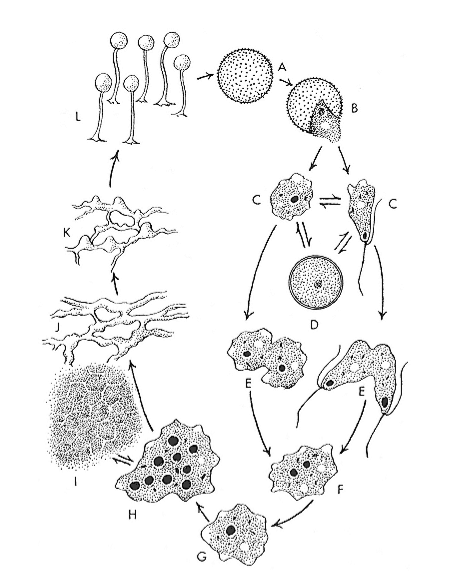
\includegraphics[width=0.5\textwidth]{./images/marco_teorico/Physarum/mixomiceto_ciclo_vida.png}
        \caption{Ciclo de vida de los mixomicetos.}
        \label{fig:MixomicetoCicloVida}
    \end{figure}
    \vskip 0.5cm
    % Parrafo 8
    Si desea profundizar en el tema, puede consultar el libro "Myxomycetes: Biology, Systematics, Biogeography, and Ecology" de Rojas \cite{Rojas2017}.
    \vskip 0.5cm